\documentclass[final]{beamer}
%% Possible paper sizes: a0, a0b, a1, a2, a3, a4.
%% Possible orientations: portrait, landscape
%% Font sizes can be changed using the scale option.
\usepackage[size=a0,orientation=portrait,scale=1]{beamerposter}

\usetheme{gemini}
\usecolortheme{seagull}
\useinnertheme{rectangles}

% ====================
% Packages
% ====================

\usepackage[utf8]{inputenc}
\usepackage{graphicx}
\usepackage{booktabs}
\usepackage{tikz}
\usepackage{tikz-3dplot}
\usetikzlibrary{3d}
\usepackage{pgfplots}
\usetikzlibrary{shapes.geometric, arrows.meta}
\usepackage{caption}
\usepackage{subcaption}
% ====================
% Lengths
% ====================
% If you have N columns, choose \sepwidth and \colwidth such that
% (N+1)*\sepwidth + N*\colwidth = \paperwidth
\newlength{\sepwidth}
\newlength{\colwidth}
\setlength{\sepwidth}{0.03\paperwidth}
\setlength{\colwidth}{0.45\paperwidth}

\newcommand{\separatorcolumn}{\begin{column}{\sepwidth}\end{column}}

% ====================
% Logo (optional)
% ====================

% LaTeX logo taken from https://commons.wikimedia.org/wiki/File:LaTeX_logo.svg
% use this to include logos on the left and/or right side of the header:
\logoleft{
\includegraphics[height=9cm]{logos/unipd.png}}
% \logoright{
\includegraphics[height=7cm]{logos/DFA.png}}

% ====================
% Footer (optional)
% ====================

\footercontent{
  CAPS 2024, Barcelona, Spain \hfill
  \insertdate \hfill
  \href{mailto:myemail@exampl.com}{\texttt{francesco.lorenzi.2@phd.unipd.it}}
}
% (can be left out to remove footer)

% ====================
% My own customization
% - BibLaTeX
% - Boxes with tcolorbox
% - User-defined commands
% ====================
% ====================
% BibLaTeX
% ====================

\usepackage[backend=biber,
	bibstyle=authoryear,
	citestyle=authoryear,
	style=authoryear,
	maxcitenames=2,
	maxbibnames=20, % limit the length of list of names (authors/editors/etc.)
	sorting=ydnt, % sort references by year (descending), name, title
	dashed=false, % show authors instead of dash in publications having the same authors
	giveninits=true % render authors' given name initials and not the full given names
]{biblatex}
%% Biblatex with Beamer bibliography icons
\setbeamertemplate{bibliography item}{%
	\ifboolexpr{ test {\ifentrytype{book}} or test {\ifentrytype{mvbook}}
		or test {\ifentrytype{collection}} or test {\ifentrytype{mvcollection}}
		or test {\ifentrytype{reference}} or test {\ifentrytype{mvreference}} }
	{\setbeamertemplate{bibliography item}[book]}
	{\ifentrytype{online}
		{\setbeamertemplate{bibliography item}[online]}
		{\setbeamertemplate{bibliography item}[article]}}%
	\usebeamertemplate{bibliography item}}
\defbibenvironment{bibliography}
{\list{}
	{\settowidth{\labelwidth}{\usebeamertemplate{bibliography item}}%
		\setlength{\leftmargin}{\labelwidth}%
		\setlength{\labelsep}{\biblabelsep}%
		\addtolength{\leftmargin}{\labelsep}%
		\setlength{\itemsep}{\bibitemsep}%
		\setlength{\parsep}{\bibparsep}}}
{\endlist}
{\item}
%% Redefine \refname
\renewcommand{\bibname}{References}
%% Redefine \parencite to use square brackets instead of braces
\DeclareCiteCommand{\parencite}
{\usebibmacro{prenote}}
{\usebibmacro{citeindex}%
	\printtext[bibhyperref]{[\usebibmacro{cite}]}}
{\multicitedelim}
{\usebibmacro{postnote}}
%% Highlight author names using Beamer data annotation
%% Usage: add a new line `author+an = {<author-order>=highlight}` to an entry
%% For example: author+an = {3=highlight} => highlight the 3rd author name
\AtBeginBibliography{
	\renewcommand*{\mkbibnamegiven}[1]{%
		\ifitemannotation{highlight}
		{\textbf{#1}}
		{#1}%
	}
	
	\renewcommand*{\mkbibnamefamily}[1]{%
		\ifitemannotation{highlight}
		{\textbf{#1}}
		{#1}%
	}
}

% ====================
% Boxes with tcolorbox
% ====================
\usepackage[most]{tcolorbox}

%%% Beamer colors in boxes

\newcommand{\beamercolorsinboxes}[1]{
	\setbeamercolor{itemize item}{fg=#1!75!black}
	\setbeamercolor{itemize/enumerate body}{fg=#1!65!white}
	\setbeamercolor{itemize/enumerate subbody}{fg=#1!65!white}
	\setbeamercolor{item projected}{fg=white, bg=#1!75!black}
}

%%% Highlight Oval Box
\newtcbox{\xmybox}[1][red]{on line,
	arc=7pt,colback=#1!10!white,colframe=#1!50!black,
	before upper={\rule[-3pt]{0pt}{10pt}},boxrule=1pt,
	boxsep=0pt,left=6pt,right=6pt,top=2pt,bottom=2pt}
%%% Box for stating problems
%%%%%%%%
%Usage: (similar for infobox)
%	\begin{defbox}{title}
	%		contents
	%	\end{defbox}
%%%%%%%%
\newtcolorbox{defbox}[1]{%
	enhanced,
	attach boxed title to top 	left={xshift=5mm,yshift=-5mm,yshifttext=-5mm},
	colback=cyan!5!white,
	colframe=cyan!75!black,
	coltitle=cyan!80!black,
%	left=0mm,right=0mm,top=2mm,bottom=0mm,
	title={#1},
	fonttitle=\bfseries\large, fontupper=\color{cyan!65!white},
	boxed title style={colback=cyan!5!white,colframe=cyan!75!black},
	before upper={
		\beamercolorsinboxes{cyan}
	}
}%
%%% Box for announcement
\newtcolorbox{infobox}[1]{%
	enhanced,
	attach boxed title to top 	left={xshift=5mm,yshift=-5mm,yshifttext=-5mm},
	colback=yellow,
	colframe=red!75!black,
	coltitle=red!75!black,
%	left=0mm,right=0mm,top=2mm,bottom=0mm,
	title={#1},
	fonttitle=\bfseries\large, fontupper=\color{red!65!white},
	boxed title style={colback=yellow,colframe=red!75!black},
	before upper={
		\beamercolorsinboxes{red}
	}
}%
%%% Box for example
\newtcolorbox{exabox}[1]{%
	enhanced,
	attach boxed title to top 	left={xshift=5mm,yshift=-5mm,yshifttext=-5mm},
	colframe=brown!75!black,colback=brown!5!white,coltitle=brown!50!brown!75!black,
%	left=0mm,right=0mm,top=2mm,bottom=0mm,
	title={#1},
	fonttitle=\bfseries\large, fontupper=\color{brown!65!white},
	boxed title style={colback=brown!5!white,coltitle=brown!50!brown!75!black},
	before upper={
		\beamercolorsinboxes{brown}
	}
}%
%%% Theorem Box
%%%%%%%%
%Usage: (similar for conjecture, lemma, etc.)
%	\begin{thm}{title}{nameref}
	%		contents
	%	\end{thm}
% Use \ref{thm:nameref} to refer to the theorem
%%%%%%%%
%%%% Use \newtcbtheorem[number within=section]{thm} to number within each section
\newtcbtheorem[]{thm}%
{Theorem}{attach boxed title to top 	left={xshift=5mm,yshift=-5mm,yshifttext=-5mm},
	enhanced jigsaw,
	%	top=2mm,bottom=0mm,left=0mm,right=0mm,
	fonttitle=\bfseries\large,fontupper=\itshape\color{blue!65!white},
	colframe=blue!75!black,colback=blue!5!white,coltitle=blue!50!blue!75!black,
	boxed title style={colback=blue!5!white,coltitle=blue!50!blue!75!black},
	before upper={
		\beamercolorsinboxes{blue}
	}
}{thm}%
%%% Proposition Box
\newtcbtheorem[use counter from=thm]{prop}%
{Proposition}{attach boxed title to top 	left={xshift=5mm,yshift=-5mm,yshifttext=-5mm},
	enhanced jigsaw,
	%	top=2mm,bottom=0mm,left=0mm,right=0mm,
	fonttitle=\bfseries\large,fontupper=\itshape,
	colframe=gray!75!black,colback=gray!5!white,coltitle=gray!50!gray!75!black,
	boxed title style={colback=gray!5!white,coltitle=gray!50!gray!75!black},
	before upper={
		\beamercolorsinboxes{gray}
	}
}{prop}%
%%% Conjecture Box
\newtcbtheorem[use counter from=thm]{conj}%
{Conjecture}{attach boxed title to top 	left={xshift=5mm,yshift=-5mm,yshifttext=-5mm},
	enhanced jigsaw,
	%	top=2mm,bottom=0mm,left=0mm,right=0mm,
	fonttitle=\bfseries\large,fontupper=\slshape,
	colframe=orange!75!black,colback=orange!5!white,coltitle=orange!50!orange!75!black,
	boxed title style={colback=orange!5!white,coltitle=orange!50!orange!75!black},
	before upper={
		\beamercolorsinboxes{orange}
	}
}{conj}%
%%% Lemma Box
\newtcbtheorem[use counter from=thm]{lem}%
{Lemma}{attach boxed title to top 	left={xshift=5mm,yshift=-5mm,yshifttext=-5mm},
	enhanced jigsaw,
	%	top=2mm,bottom=0mm,left=0mm,right=0mm,
	fonttitle=\bfseries\large,fontupper=\itshape,
	colframe=green!75!black,colback=green!5!white,coltitle=green!50!green!75!black,
	boxed title style={colback=green!5!white,coltitle=green!50!green!75!black},
	before upper={
		\beamercolorsinboxes{green}
	}
}{lem}%
%%% Claim Box
\newtcbtheorem[use counter from=thm]{clm}%
{Claim}{attach boxed title to top 	left={xshift=5mm,yshift=-5mm,yshifttext=-5mm},
	enhanced jigsaw,
	%	top=2mm,bottom=0mm,left=0mm,right=0mm,
	fonttitle=\bfseries\large,fontupper=\itshape,
	colframe=pink!75!black,colback=pink!5!white,coltitle=pink!50!pink!75!black,
	boxed title style={colback=pink!5!white,coltitle=pink!50!pink!75!black},
	before upper={
		\beamercolorsinboxes{pink}
	}
}{clm}%

%% Reference Sources
\addbibresource{refs.bib}
\renewcommand{\pgfuseimage}[1]{\includegraphics[scale=2.0]{#1}}

\title{Scattering of matter-wave soliton from a narrow barrier:
transmission coefficient and induced collapse}

\author{\underline{Francesco Lorenzi} \inst{1} \and Luca Salasnich \inst{2}}

\institute[shortinst]{\inst{1} Dipartimento di Fisica e Astronomia ”Galileo Galilei”, Università di Padova (Italy)\samelineand \inst{2} Instituto Nazionale di Fisica Nucleare (INFN), Sezione di Padova (Italy)  \\
\inst{3} Padua Quantum Technology Research Center, Università di Padova (Italy) \samelineand                        
\inst{4} Instituto Nazionale di Ottica del Consiglio Nazionale delle Ricerche (INO-CNR) (Italy)}

\date{January 25, 2024}

%%% DOCUMENT
\begin{document}
\begin{frame}[t]
  
  %%% INTRO BLOCK
  \begin{columns}[t]
  \begin{column}{2\colwidth+\sepwidth}
  \begin{block}{Introduction}
    \begin{minipage}{35cm}
      We consider a ultracold Bose gas trapped in a \textbf{quasi one-dimensional} setting.
      \begin{itemize}
        \item  By using the three-dimensional Gross-Pitaevskii equation, we numerically obtain the dynamics of the collision of a matter-wave soliton with a narrow potential barrier.
        \item We determine how the \textbf{transmission coefficient} depends on the soliton impact velocity and the barrier height.
        \item We also obtain the regions of parameters where there is the \textbf{collapse} of the bright soliton induced by the collision.
        \item We compare the three-dimensional results with the ones obtained by \textbf{three different} one-dimensional nonlinear Schrödinger equations.
      \end{itemize}
    \end{minipage}\hspace{1cm}%
    \begin{minipage}{35cm}
      \begin{figure}
        \subfloat[$v=0.5$]{%
        {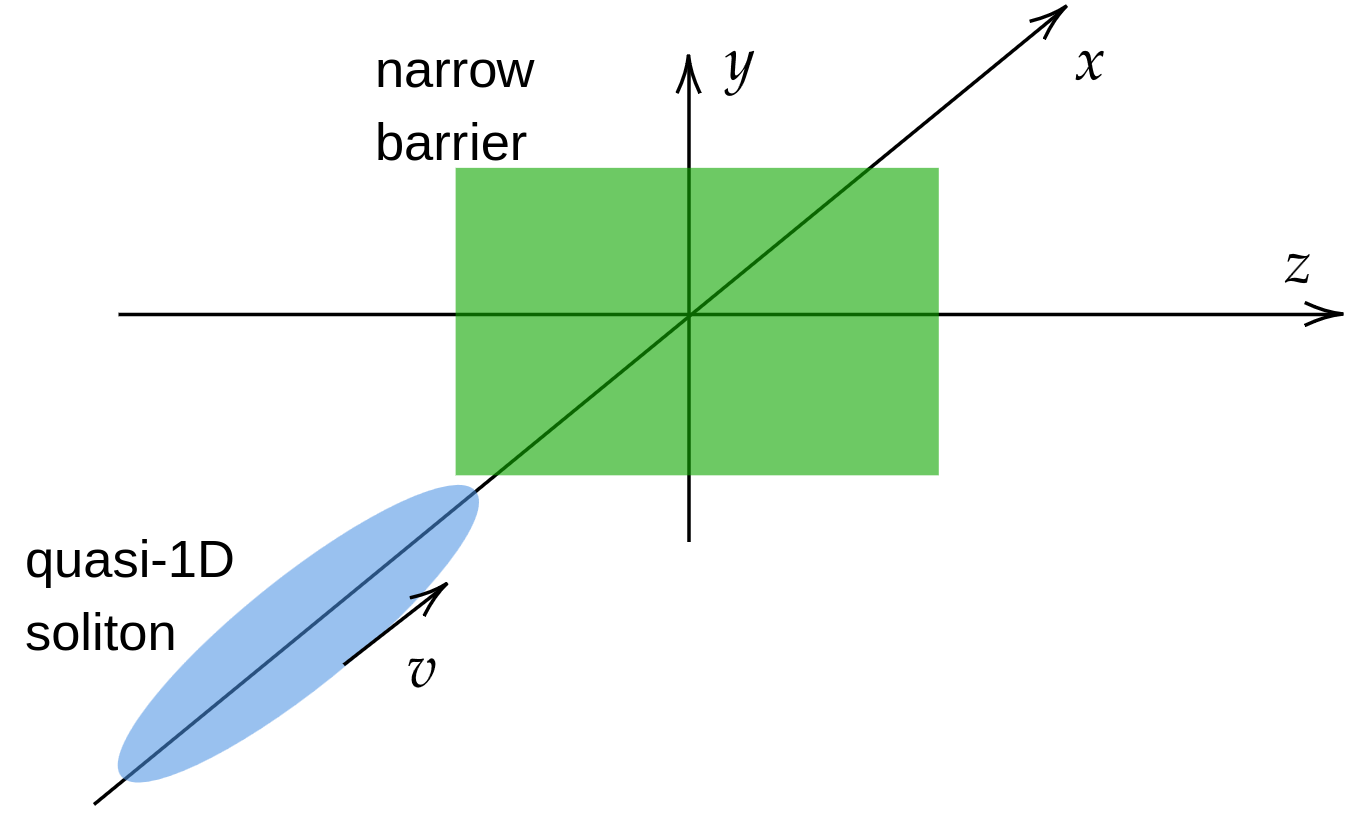
\includegraphics[width=0.4\linewidth]{figures/barrier.png}}%
        }\hspace{2cm}
      \subfloat[$v=1$]{%
        {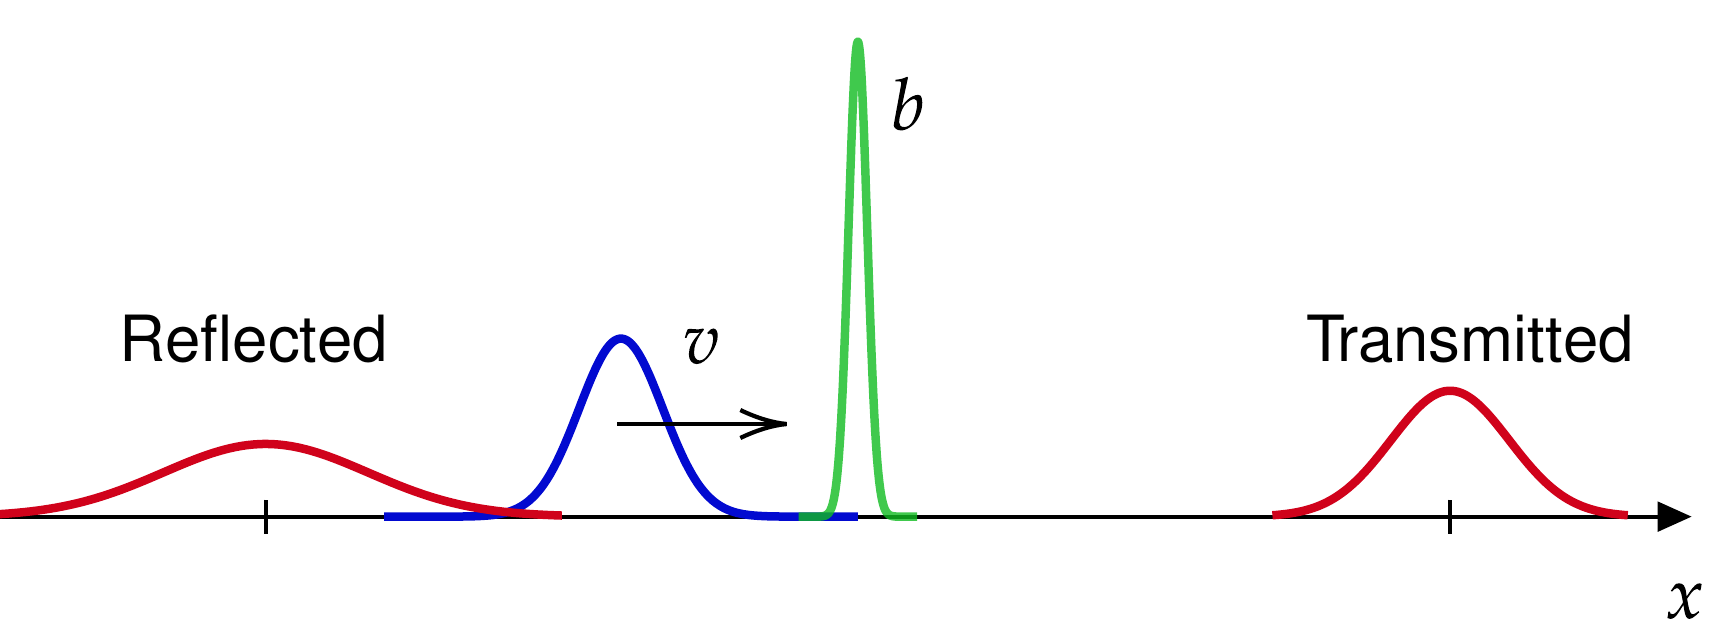
\includegraphics[width=0.4\linewidth]{figures/solitoni.png}}%
      }
    \end{figure}
    \end{minipage}\hspace{1cm}% 
    %
    \begin{minipage}{20cm}
      \begin{equation}\label{eq:3dgpe}
        i\hbar \dfrac{\partial}{\partial t}\psi = \left[-\dfrac{\hbar^2}{2m} \nabla^2 + U  + g(N-1)|\psi|^2\right]\psi.
      \end{equation}
      \begin{equation}
        U(x, y, z) = \frac{1}{2}m\omega_\perp^2 (y^2+z^2) + V(x),
      \end{equation}
    \end{minipage}
    
  \end{block}
  \end{column}
  \end{columns}


  %%% MAIN BLOCKS
  \begin{columns}[t]
    \separatorcolumn
    %%% LEFT COLUMN
    \begin{column}{\colwidth}
      
      %%% COLLISION
      \begin{block}{Dynamics at the collision}
        When a one-dimensional soliton impinge on a narrow barrier, the transmission coefficient $T$ is expected to be a \textbf{discontinuous function} of $v$, the impinging velocity, and $b$, the barrier energy, for sufficiently low values of the parameters. As shown in a previous work, collapse can be initiated [MALOMED] by the collision event, so it is important to distinguish between static and dynamic collapse.
        \begin{figure}
          \subfloat[$v=0.5$]{%
          {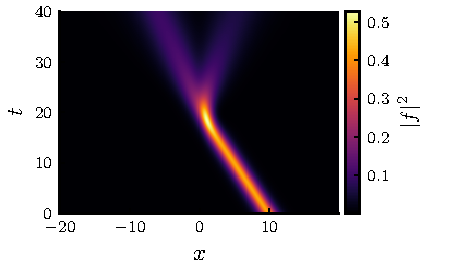
\includegraphics[width=.30\linewidth]{figures/PSI__10_4.7.pdf}}%
          }\hspace{2cm}
        \subfloat[$v=1$]{%
          {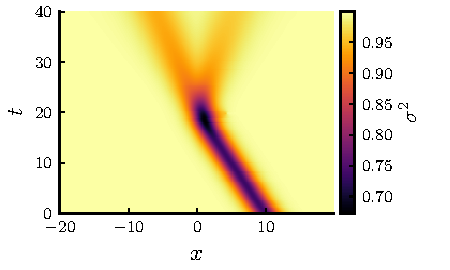
\includegraphics[width=.30\linewidth]{figures/SIGMA10_4.7.pdf}}%
        }
      \end{figure}
      \end{block}

      %%% REDUCTION
      \begin{exampleblock}{Dimensional reduction strategies for the Gross-Pitaevskii equation}{}
        
        Starting from the GP Lagrangian in 3D:
        \begin{equation}\label{eq:3dlagrangian}
        \mathcal{L}= \int d^3 \mathbf{r} \ \psi^* \left[i \hbar \frac{\partial}{\partial t}+\frac{\hbar^2}{2 m} \nabla^2-U-\frac{g}{2}(N-1)|\psi|^2 \right] \psi,
        \end{equation}
        with   
        \begin{equation}
          g = \frac{4\pi \hbar^2 a_s}{m},
        \end{equation}
        one can compute the corresponding Euler-Lagrange equation:

        \heading{ciao}
        \begin{equation}
          V(x; \ b) = b \ \exp[-\frac{x^2}{2 w^2}].
        \end{equation}


          A better approach is to assume a \textbf{variable transverse width} 
        \begin{equation}
            \phi(y, z, \sigma(x, t)) = \dfrac{1}{\sqrt{\pi} \sigma(x, t)} \exp\left[-\frac{y^2+z^2}{2\sigma(x, t)^2}\right]
        \end{equation}
        Writing the 3D GP Lagrangian, we may hope to integrate along the transverse variables

          Integrating the term proportional to $\frac{\partial}{\partial t} \sigma$ gives $0$, as one may realize by looking at the symmetry of its prefactor. However, the term proportional to $\frac{\partial^2}{\partial x^2} \phi$ gives a non-null contribution to the 1D Lagrangian.
           
          Let us now consider the corresponding Euler-Lagrange equations. These will be computed for $f$ and $\sigma$, thus $\sigma$ is a proper variational parameter, and constitute a set of coupled PDE and ODE.
          
   
      \end{exampleblock}

      \begin{block}{One dimensional effective equations}

        The simplest dimensional reduction
        \begin{equation}
          \text{GPE:} \qquad i\hbar \frac{\partial}{\partial t} f = \left[-\dfrac{\hbar^2}{2m} \frac{\partial}{\partial x}^2  + V + \hbar\omega_\perp+ \dfrac{N-1}{2\pi \sigma^2} g|f|^2 \right]
        \end{equation}
        The effective equations that are compared are \large{NPSE}
        \begin{equation}
          \text{NPSE:}\left\{\begin{split}
              &i\hbar \frac{\partial}{\partial t} f = \left[-\dfrac{\hbar^2}{2m} \frac{\partial}{\partial x}^2  + V +\dfrac{\hbar^2}{2m}\dfrac{1}{\sigma^{2}}  + \dfrac{m\omega_\perp^2}{2}\sigma^2 + \dfrac{N-1}{2\pi \sigma^2} g|f|^2 \right] \\
          &- m\omega_\perp^2\sigma + \left[\dfrac{\hbar^2}{m} + \dfrac{N-1}{2\pi} g|f|^2\right]\sigma^{-3} +\frac{\hbar^2}{m} \sigma^{-3}\left(\sigma\frac{\partial}{\partial x}^2 \sigma - \left(\frac{\partial}{\partial x} \sigma \right)^2 \right)= 0.
        \end{split} \right.
        \end{equation} 
        \large{NPSE+}
     \begin{equation}
          \text{NPSE+:}\left\{\begin{split}
              &i\hbar \frac{\partial}{\partial t} f = \left[-\dfrac{\hbar^2}{2m} \frac{\partial}{\partial x}^2  + V +\dfrac{\hbar^2}{2m}\dfrac{1}{\sigma^{2}}  + \dfrac{m\omega_\perp^2}{2}\sigma^2 + \dfrac{N-1}{2\pi \sigma^2} g|f|^2 \right] \\
          &- m\omega_\perp^2\sigma + \left[\dfrac{\hbar^2}{m} + \dfrac{N-1}{2\pi} g|f|^2\right]\sigma^{-3} +\frac{\hbar^2}{m} \sigma^{-3}\left(\sigma\frac{\partial}{\partial x}^2 \sigma - \left(\frac{\partial}{\partial x} \sigma \right)^2 \right)= 0.
        \end{split} \right.
        \end{equation}

      \end{block}
      \begin{block}{Soliton-like solutions}
          \begin{figure}
            \subfloat[$v=0.5$]{%
            {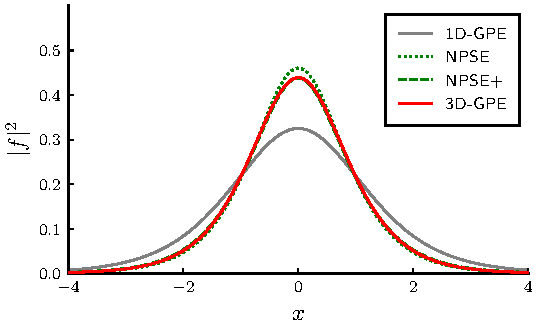
\includegraphics[width=.40\linewidth]{figures/fig1_0.65_ground_states.pdf}}%
          }
          \subfloat[$v=1$]{%
            {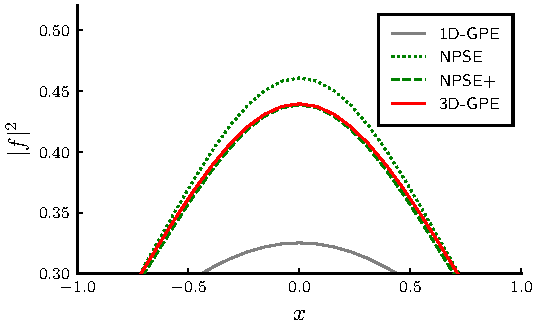
\includegraphics[width=.40\linewidth]{figures/fig2_0.65_ground_states_zoom.pdf}}%
          }
        \end{figure}
        \begin{figure}x
            \subfloat[$v=0.5$]{%
            {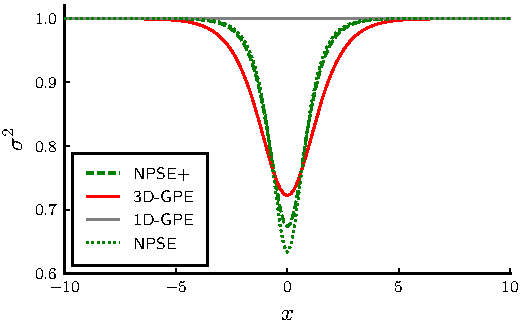
\includegraphics[width=.40\linewidth]{figures/fig3_compare_sigma2_065.pdf}}%
          }
          \subfloat[$v=1$]{%
            {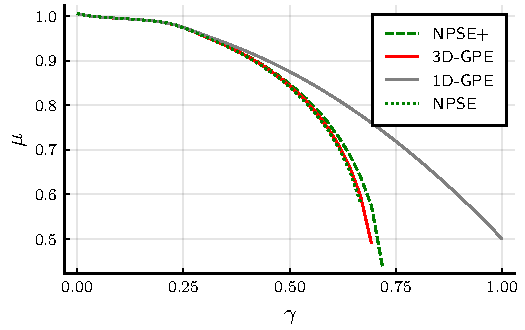
\includegraphics[width=.40\linewidth]{figures/fig4_mu.pdf}}%
          }
        \end{figure}
      \end{block}

    \end{column}
    \separatorcolumn
    %%% RIGHT COLUMN
    \begin{column}{\colwidth}

      %%% NUMERICAL
      \begin{block}{Numerical methods}
        % The time-marching scheme we use for all the simulations is the SSFM, adopting Strang splitting of the nonlinear and linear part of the evolution operator. The SSFM is well-known to be accurate to the second order in time and to every order in space, thus being highly efficient in the spatial discretization. The drawback of the method - or the feature, depending on the point of
        % view - is to natively implement PBC. The implementation of absorption boundaries is still possible but not straightforward.
        We assume the field to be localized away from the boundary in order to neglect this problem. The time step in both setups is chosen to be $h_t = 0.01$. These parameters have been proven to give a total truncation error in the $L_\infty$ norm of the order of $10^{-4}$, and allow for a reasonable computation time of all the calculations.
        The ground state solutions are computed using an imaginary-time propagation method. We point out that some modifications of this method are available under the name of normalized gradient-flow methods.

        We have an isotropic confinement, in which we have units: \textbf{energy} $\longrightarrow$ $\hbar\omega_\perp$, \textbf{time}  $\rightarrow$ $\omega_\perp^{-1}$, \textbf{length} $\longrightarrow$ $l_\perp$.

        \begin{itemize}
            \item 1D simulations a total length of $L = 40$, with a grid of $N = 512$ points.
            \item  3D simulations, we use a grid of $(N_x, N_y, N_z) = (512, 40, 40)$ points, with  total lengths of $(L_x, L_y, L_z) = (40, 10, 10)$.
        \end{itemize}
        Collapse threshold is set to a probability per point of $0.3$.
          The time step in both setups is chosen to be $h_t = 0.01$. These parameters have been proven to give a total truncation error in the $L_{\infty}$ norm of the order of $10^{-4}$, and allow for a reasonable computation time of all the calculations.
      \end{block}


      \begin{block}{Results}
        \begin{figure}
          \centering
          \subfloat[3D-GPE]{%
            {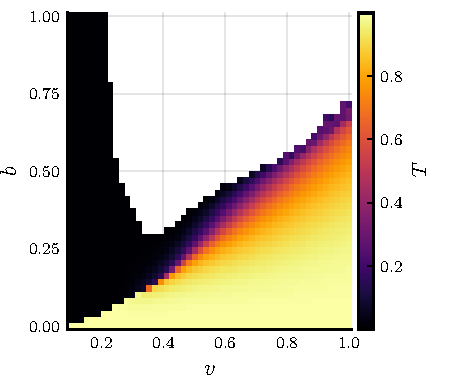
\includegraphics[width=.40\linewidth]{figures/tiles_G3.pdf}}%
          }%
          \subfloat[NPSE+]{%
            {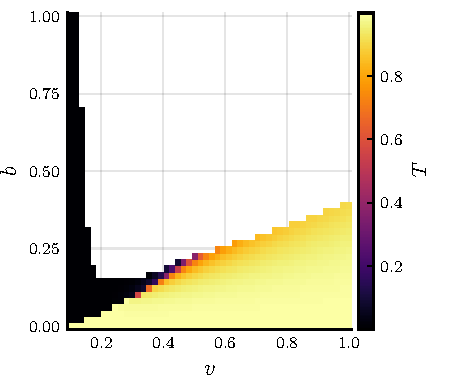
\includegraphics[width=.40\linewidth]{figures/tiles_N-1.pdf}}%
          }
          
          \subfloat[NPSE]{%
            {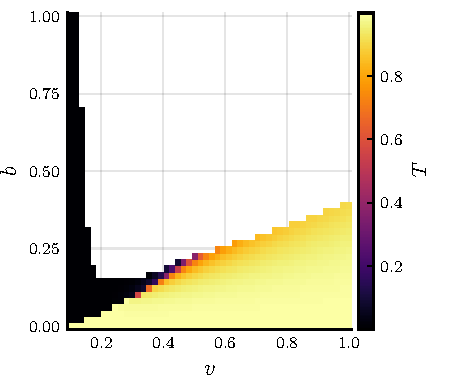
\includegraphics[width=.40\linewidth]{figures/tiles_N-1.pdf}}%
          }
          \subfloat[1D-GPE]{%
            {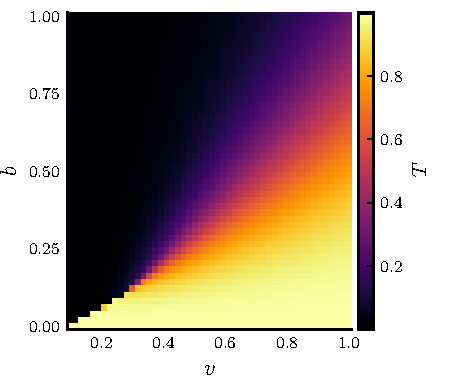
\includegraphics[width=.40\linewidth]{figures/tiles_G1.pdf}}%
          }
          \caption{Comparison of the transmission coefficient and the collapse regions for the various equations. $v$ is in units of $\sqrt{\hbar \omega_\perp / m}$, $b$ is in units of $\hbar \omega_\perp$.}
          \label{fig:heatmap}
        \end{figure}
        \begin{figure}
            \subfloat[$v=0.5$]{%
            {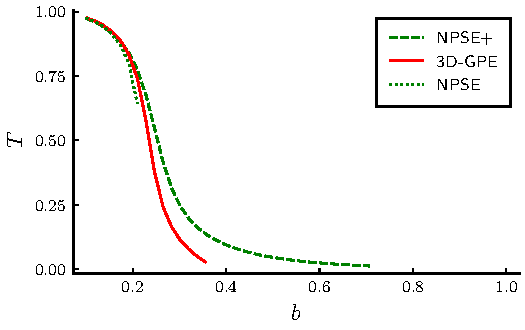
\includegraphics[width=.40\linewidth]{figures/fig8_collapse.pdf}}%
          }
          \subfloat[$v=1$]{%
            {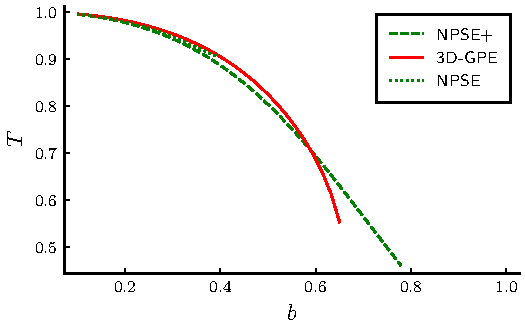
\includegraphics[width=.40\linewidth]{figures/fig9_collapse.pdf}}%
          }
        \end{figure}
      \end{block}

      \begin{block}{Conclusions and perspectives}
        We investigated how the choice of \textbf{dimensional reduction} impacts the description of some features of the process, namely the transmission coefficient and the onset of barrier-induced collapse, also using the familiar one-dimensional Gross-Pitaevskii. We first reviewed the \textbf{ground state properties} given by all the schemes, highlighting the role of the variational transverse width. Then we compared the scattering properties: our results show that by using the NPSE in a regime of high barrier energy and high velocity it \textbf{fails to describe the 3D dynamics} due to the vanishing of the transverse width of the solution. Our main result is that by adopting a slight modification of the transverse width using the \textbf{true variational} solution with the NPSE ansatz, the method has a good agreement with the 3D-GPE.
      \end{block}
      \begin{block}{References}
        \printbibliography[heading=none]          
        \begin{enumerate}
            \item Khaykovich, L. and Malomed, B. A. Deviation from one dimensionality in stationary properties and collisional dynamics of matter-wave solitons. Phys. Rev. A 74, 023607 (2006).
            \item  Salasnich, L., Parola, A. and Reatto, L. Effective wave equations for the dynamics of cigar-shaped and disk-shaped Bose condensates. Phys. Rev. A 65, 043614 (2002).
            \item Cuevas, J., Kevrekidis, P. G., Malomed, B. A., Dyke, P. and Hulet, R. G. Interactions of solitons with a gaussian barrier: splitting and recombination in quasi-one-dimensional and three-dimensional settings. New J. Phys. 15, 063006 (2013). 
            \item Helm, J. L., Rooney, S. J., Weiss, C. and Gardiner, S. A. Splitting bright matter-wave solitons on narrow potential barriers: Quantum to classical transition and applications to interferometry. Phys. Rev. A 89, 033610 (2014)
            \item Lorenzi, F. SolitonDynamics.jl \textit{GitHub repository} \texttt{github.com/lorenzifrancesco/CondensateDynamics.jl} (2023).
            \item Wang, C.-H., Hong, T.-M., Lee, R.-K. and Wang, D.-W. Particle-wave duality in quantum tunneling of a bright soliton. Opt. Expr. 20, 22675–22682 (2012).
        \end{enumerate}
      \end{block}

    \end{column}
    \separatorcolumn
  \end{columns}
\end{frame}
\end{document}
